% Full-width rows keep all three methods legible while preserving fixed order.
\newcommand{\BookExampleRow}[2]{%
  \multicolumn{3}{c}{\textbf{#1}} \\[2pt]
  \includegraphics[
    width=0.29\textwidth,height=0.145\textheight,keepaspectratio]
    {figures/flux_#2.png} &
  \includegraphics[
    width=0.29\textwidth,height=0.145\textheight,keepaspectratio]
    {figures/baseline_#2.png} &
  \includegraphics[
    width=0.29\textwidth,height=0.145\textheight,keepaspectratio]
    {figures/informative_#2.png} \\[7pt]
}

\begin{figure*}[p]
  % Keep the appendix heading with its first full-width illustration.
  \begin{minipage}{\textwidth}
    \section{Unedited Output Examples}
    \label{app:examples}
    Figures~\ref{fig:unedited-comparison-first} and
    \ref{fig:unedited-comparison-second} show all eight current subjects in
    fixed list order. The FLUX and SD1.5 columns are the same saved outputs
    measured in Table~\ref{tab:image-results}. The Informative Drawings column
    was generated later, once per same saved portrait, using the released
    \emph{anime\_style} checkpoint and is included only for qualitative
    context. Every output is shown; scaling is solely for presentation, with
    no reranking or image correction. Figure~\ref{fig:unedited-book-page}
    remains the unchanged first book page.
  \end{minipage}\par\vspace{10pt}
  \centering
  \small
  \begin{tabular}{@{}ccc@{}}
    \textbf{FLUX} & \textbf{SD1.5 baseline} &
      \textbf{Informative Drawings} \\[3pt]
    \BookExampleRow{Otto Hahn}{Otto_Hahn}
    \BookExampleRow{Robert Bunsen}{Robert_Bunsen}
    \BookExampleRow{Emil von Behring}{Emil_von_Behring}
    \BookExampleRow{Jacob Grimm}{Jacob_Grimm}
  \end{tabular}
  \caption{All-case visual comparison for current subjects 1--4. FLUX and
    SD1.5 are the evaluated outputs; Informative Drawings is a post-hoc
    qualitative comparator. All three columns use the same saved source
    portraits with method-specific preprocessing. The exact generated files
    are scaled only for presentation; no reranking, correction, or human
    rating is represented.}
  \label{fig:unedited-comparison-first}
\end{figure*}

\begin{figure*}[p]
  \centering
  \small
  \begin{tabular}{@{}ccc@{}}
    \textbf{FLUX} & \textbf{SD1.5 baseline} &
      \textbf{Informative Drawings} \\[3pt]
    \BookExampleRow{Hannah Arendt}{Hannah_Arendt}
    \BookExampleRow{K. Ferdinand Braun}{K._Ferdinand_Braun}
    \BookExampleRow{Alfred Wegener}{Alfred_Wegener}
    \BookExampleRow{Boris Pasternak}{Boris_Pasternak}
  \end{tabular}
  \caption{All-case visual comparison for current subjects 5--8, continuing
    the fixed order. FLUX and SD1.5 are the evaluated outputs; Informative
    Drawings is a post-hoc qualitative comparator. All three columns use the
    same saved source portraits with method-specific preprocessing. Exact
    generated files are scaled only for presentation; no reranking,
    correction, or human rating is represented.}
  \label{fig:unedited-comparison-second}
\end{figure*}

\begin{figure*}[p]
  \centering
  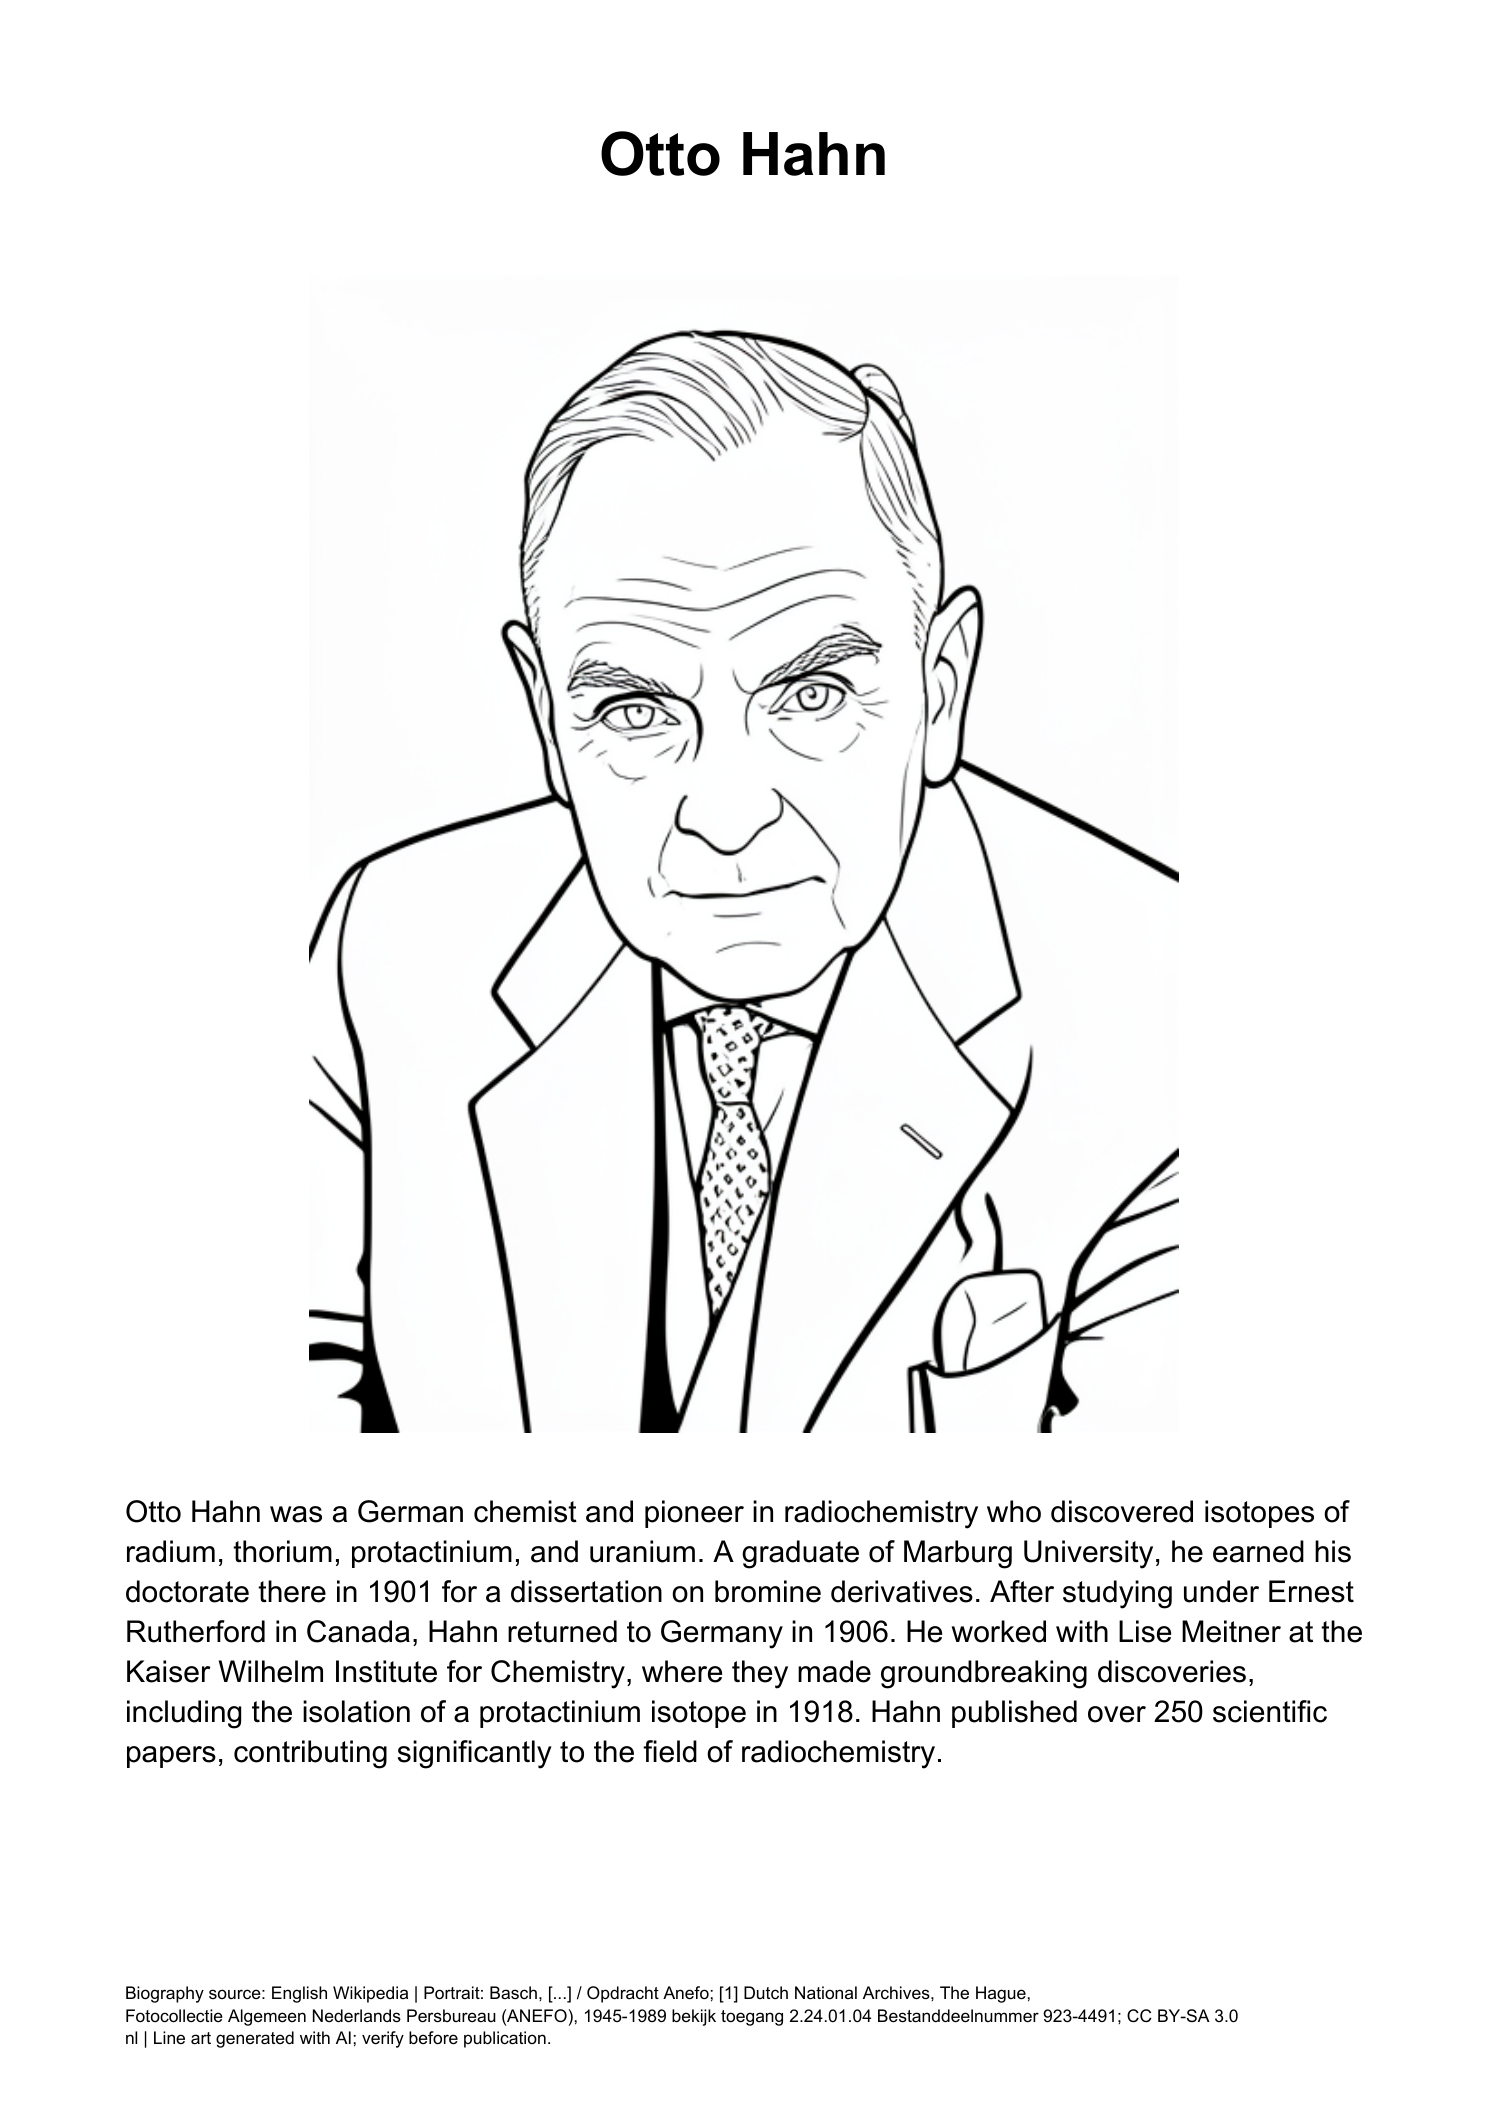
\includegraphics[width=0.93\textwidth,height=0.85\textheight,keepaspectratio]
    {figures/generated_page.png}
  \caption{The unchanged first page of the generated eight-page book,
    featuring Otto Hahn, the first current subject. The complete original
    page was mechanically rendered at 180 dpi and scaled for presentation;
    its biography, portrait, layout, source link, and attribution remain as
    generated. It is an illustrative document output, not a manually polished
    educational page or evidence of human preference.}
  \label{fig:unedited-book-page}
\end{figure*}
